\chapter{Projektformulering (Alle)}

\section{Version}
\begin{table}[h]
	\centering
	\begin{tabularx}{\textwidth}{|l|l| l|X|}
	\hline
	Dato	& Version	& Initialer & Ændring	\\ \hline
	8. oktober & 1 & KT	& Første udkast af dokumentet efter review \\ \hline
	\end{tabularx}
\end{table}

Vores mål med dette projekt er at udvikle et home automation system, som kan simulering tilstedeværelse i en bolig. Gennem styring af de tilkoblede enheder, som fx TV, lys og radio, kan udefrakommende ledes til at tro, at der er nogen tilstede, selvom brugeren ikke er hjemme. Udover home security vil systemet også kunne hjælpe brugeren i dagligdagen ved at automatisere visse aspekter af hverdagen, fx ved at indstille et fast tidspunkt for aktivering af radio om morgenen eller mulighed for at tænde og styre TV. Systemet er tilpasset én bestemt bruger og dennes særlige behov. Brugeren er en familie, hvor alle er beskæftigede i dagstimerne og derfor vil sikre sig mod tyveri. Familien er ofte på ferie og er generelt meget hjemmefra. Når de endelig er hjemme, vil de gerne have en mere automatiseret hverdag i deres hjem. Familien kan via systemet styre to lamper, et TV og en radio. 

Brugeren kan via systemet styre følgende funktioner i enhederne:
\begin{itemize}
\item TV:
\begin{itemize}
\item Tænde- og slukkefunktion
\item Skifte kanal (op/ned)
\item Justere volumen 
\item Valg af specifikt kanalnummer
\end{itemize}

\item Radio:
\begin{itemize}
\item Tænde og slukke
\item Kanalsøgning (op/ned)
\item Justere volumen
\item Valg af forudindstillet kanal
\end{itemize}

\item Belysning:
\begin{itemize}
\item Tænde og slukke enkeltvis
\item Justere lysintensitet enkeltvis
\end{itemize}
\end{itemize}

Disse enheders funktioner kan herefter indstilles af brugeren via den centrale computer til at ske ved bestemte tidspunkter ved at konfigurere eller vælge forudbestemte scenarier. Disse scenarier har en varighed på 24 timer og gentages automatisk indtil de stoppes.
For at forhindre uatoriseret adgang til systemets brugerflade er systemet beskyttet med en kodelås, som brugeren selv ved tidligere lejlighed har indstillet.

Systemet består af:
\begin{itemize}
\item Software til installation på brugerens PC
\item En X.10 transmitter-controller, bestående af et STK500 kit samt et X.10 interface
\item Fire X.10 receiver-controllere, bestående af STK500 kit samt X.10 interface
\item En kodelås på et Altera DE2 udviklingsboard
\end{itemize}

Systemet er forbundet til det eksisterende elnet i hjemmet via X.10 controllerne. Brugeren indstiller alting via softwaren på sin PC, som gemmer brugerens preferencer på transmittereren. Denne skal være koblet til både kodelås samt X.10 interfacet og sørger for at afvikle det indstillede program, selv når brugerens PC er slukket. For hver enhed der skal styres, er der en specifik receiver-controller, som undstøtter den tilkoblede enhed. For radio og TV receiver-controllerne er der på hver koblet en IR-transmitter på, som styres af det pågældende STK500 kit. Dette sikrer kommunikation til radio/TV. Controllerne er hver især tilkoblet elnettet og deres respektive enheder. Hele denne opsætning kan ses i Figur \ref{fig:kommunikation}.

\begin{figure}[h]
\centering
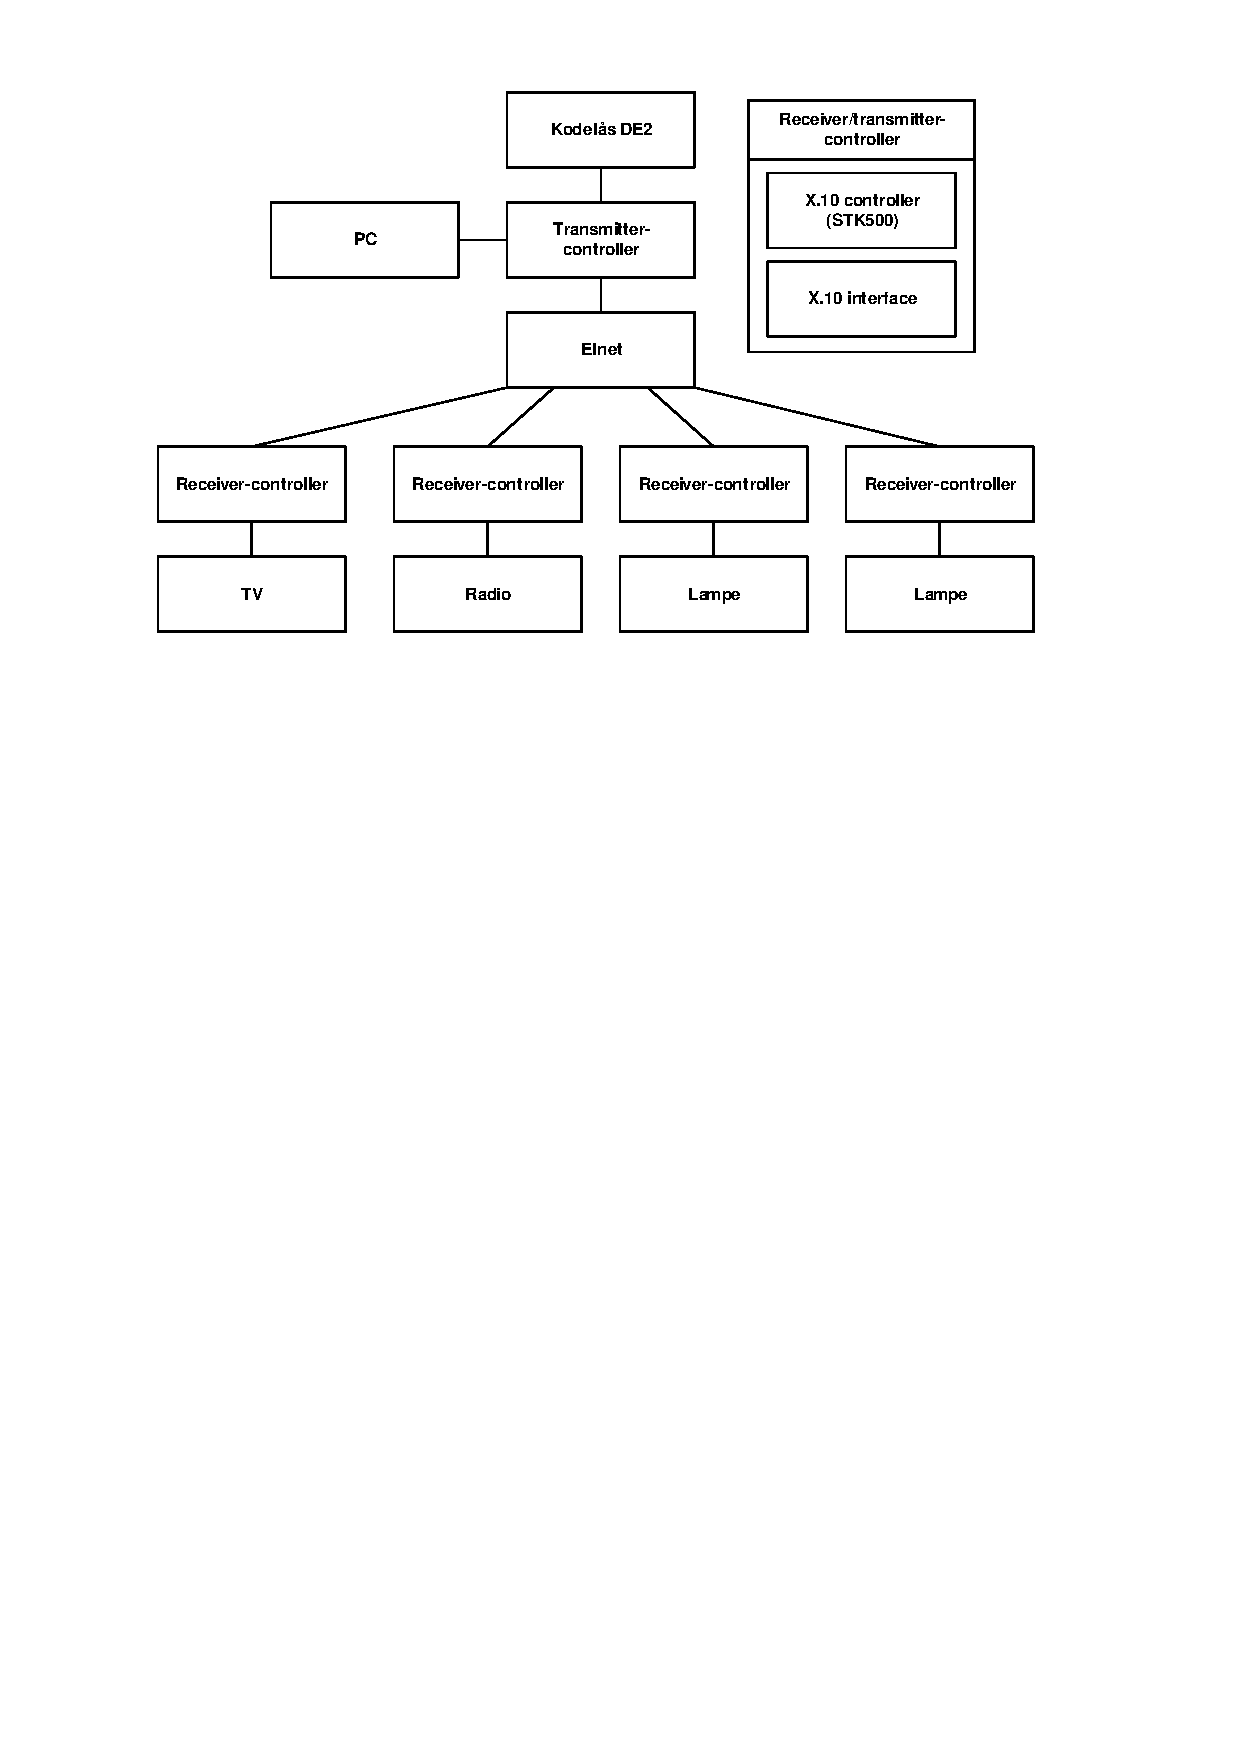
\includegraphics[scale=1,trim=50 535 80 30, clip=true]{../Projektformulering/kommunikation_diagram}
\caption{Kommunikationsveje mellem enheder i systemet}
\label{fig:kommunikation}
\end{figure}

\clearpage